%%%%%%%%%%%%%%%%%%%%%%%%%%%%%%%%%%%%%%%%%
% FRI Data Science_report LaTeX Template
% Version 1.0 (28/1/2020)
%
% Jure Demšar (jure.demsar@fri.uni-lj.si)
%
% Based on MicromouseSymp article template by:
% Mathias Legrand (legrand.mathias@gmail.com)
% With extensive modifications by:
% Antonio Valente (antonio.luis.valente@gmail.com)
%
% License:
% CC BY-NC-SA 3.0 (http://creativecommons.org/licenses/by-nc-sa/3.0/)
%
%%%%%%%%%%%%%%%%%%%%%%%%%%%%%%%%%%%%%%%%%


%----------------------------------------------------------------------------------------
%	PACKAGES AND OTHER DOCUMENT CONFIGURATIONS
%----------------------------------------------------------------------------------------
\documentclass[fleqn,moreauthors,10pt]{ds_report}
\usepackage[english]{babel}

\graphicspath{{fig/}}




%----------------------------------------------------------------------------------------
%	ARTICLE INFORMATION
%----------------------------------------------------------------------------------------

% Header
\JournalInfo{UL FRI Data Science - Natural Language Processing, 2021-2022}

% Interim or final report
\Archive{Interim report}
%\Archive{Project Report}

% Article title
\PaperTitle{Literacy situation models knowledge base creation}

% Authors and their info
%\Authors{John Doe\textsuperscript{1}}
%\affiliation{\textsuperscript{1}\textit{john.doe@fri.uni-lj.si, 63181234}}

% Multiple authors
\Authors{Uroš Škrjanc\textsuperscript{1}, Matthew Tanti\textsuperscript{2}, and Marko Novak\textsuperscript{3}}
\affiliation{\textsuperscript{1}\textit{us1883@student.uni-lj.si, 63030323}}
\affiliation{\textsuperscript{2}\textit{mt9734@student.uni-lj.si, 63210511}}
\affiliation{\textsuperscript{3}\textit{mn3983@student.uni-lj.si, 63130166}}

% Keywords
\Keywords{story entities, family relationship extraction, short stories}
\newcommand{\keywordname}{Keywords}


%----------------------------------------------------------------------------------------
%	ABSTRACT
%----------------------------------------------------------------------------------------

\Abstract{
%The abstract goes here. The abstract goes here. The abstract goes here. The abstract goes here. The abstract goes here. The abstract goes here. The abstract goes here. The abstract goes here. The abstract goes here. The abstract goes here. The abstract goes here. The abstract goes here. The abstract goes here. The abstract goes here. The abstract goes here. The abstract goes here. The abstract goes here. The abstract goes here. The abstract goes here. The abstract goes here. The abstract goes here. The abstract goes here. The abstract goes here. The abstract goes here. The abstract goes here. The abstract goes here.
}

%----------------------------------------------------------------------------------------

\begin{document}

% Makes all text pages the same height
\flushbottom

% Print the title and abstract box
\maketitle

% Removes page numbering from the first page
\thispagestyle{empty}

%----------------------------------------------------------------------------------------
%	ARTICLE CONTENTS
%----------------------------------------------------------------------------------------

\section*{Introduction}

The field of recognising the content and structure of texts and extracting content from them is increasingly related to machine learning methods. Not only syntax checking but also pure understanding of texts by humans is interesting for machine learning for different motives. There is practically no more field related to language that in some way could not be linked to machine learning methods.



%These latex files are intended to serve as a the template for the FRI Data Science Project Competition. If you find mistakes in the template or have problems using it, please consult Jure Demšar (\href{mailto:jure.demsar@fri.uni-lj.si}{jure.demsar@fri.uni-lj.si}).

%In the Introduction section you should write about the relevance of your work (what is the purpose of the project, what will we solve) and about related work (what solutions for the problem already exist). Where appropriate, reference scientific work conducted by other researchers. For example, the work done by Demšar et al. \cite{Demsar2016BalancedMixture} is very important for our project. The abbreviation et al. is for et alia, which in latin means and others, we use this abbreviation when there are more than two authors of the work we are citing. If there are two authors (or if there is a single author) we just write down their surnames. For example, the work done by Demšar and Lebar Bajec \cite{Demsar2017LinguisticEvolution} is also important for successful completion of our project.


%------------------------------------------------

\section*{Methods}

In the group, we decided to try to analyse different short stories to extract information about the characters who appear in the texts and to find out what kind of relationships these characters are in.

First we found a collection of english short stories and choose a subset of them for training. Then, in the python programming language, we will use libraries such as NLTK, SpaCy, SNER, GATE... to determine which characters appear in the stories. At this stage, it will be necessary to extract the characters' actual names from the text and ensure that the correct numbers of characters and their positions in the text are extracted.

In the second part, we will try to make a model that properly connects characters in pairs into family relations. The model should determine whether a couple of characters are in a family relationship and, if so, then determine the type of relation. Due to complexity of the task, we decided not to classify realtions, that are not family related.We thnik that discovering family relations task is complex enoguh.

As part of the task, we will review the models that have already been implemented and, based on the results of the solutions already made, make our own model that would classify as accurately as possible.


%Use the Methods section to describe what you did an how you did it -- in what way did you prepare the data, what algorithms did you use, how did you test various solutions ... Provide all the required details for a reproduction of your work.

%Below are \LaTeX examples of some common elements that you will probably need when writing your report (e.g. figures, equations, lists, code examples ...).

\section*{Existing solutions}

The use of deep neural networks is on the rise in already implemented solutions, but other approaches and combinations of these are also used in models for classifying family relations between persons in the text, such as rule-based approaches, utterance attribution and vocative detection technique and unsupervised approach to the extraction of interpersonal relations are described in the articles, which we intend to take as a basis for further work. \cite{caselli2017event} \cite{nahatame2020revisiting} \cite{trabasso1985causal} \cite{mostafazadeh2016corpus} \cite{dasgupta2018automatic} \cite{mcnamara2012coh} \cite{zwaan1995dimensions} \cite{zwaan1999situation}

\section*{Relations}

We decided to check if the following relations occur between the character in short stories:
\begin{itemize}
\itemsep0em
\item Wife
\item Husband
\item Mother
\item Father
\item Daughter
\item Son
\item Sister
\item Brother
\item Grandmother
\item Grandfather
\item Granddaughter
\item Grandson
\item Mother-in-law
\item Father-in-law
\item Daughter-in-law
\item Son-in-law
\item Sister-in-law
\item Brother-in-law
\item Aunt
\item Uncle
\item Niece
\item Nephew
\item Cousin
\end{itemize}

This is the broadest family relations model we intend to use. We expect that there will be no need to add new relationships. If the model proves to be too large for our task, some relations can be removed from model.

\section*{Model}

For extracting and classification family relatins in short stories, we are considering two models: CasRel\cite{wei2020CasRel} and DocuNetl\cite{ijcai2021-551}.

CasRel is sentence oriented. This means, that in first step model discovers identities and in second step applies relation specific taggers to simultaneously identify all possible relations and the corresponding object. Relations are represented with relational triples (subject, relation, object). Model takes all subjects in sentence and for each subject iterates through relations and tries to find object, that is in appropriate relation with actual subject. Model implements more holistic approach to relation classification than usual and according to article\cite{wei2020CasRel} it achieved high accuracy on NYT and WebNLG datasets.

On the other hand, DocuNET (Document U-shaped Network) is document oriented. This means, that model tries to find relations between entities over all document. According to the article\cite{ijcai2021-551}, above 40,7\% of relations can only be identified by at the document level and model is first approach that uses implements relation extraction as semantic segmentation. Approach is similar than in computer vision, where each pixel is classified in one visual object. On the same principle DocuNET tries to classify two entities in a relation, that is defined.

We think that, because of the document level orientation, second model would be more appropriate for our task.



%\subsection*{Equations}

% You can write equations inline, e.g. $\cos\pi=-1$, $E = m \cdot c^2$ and $\alpha$, or you can include them as separate objects. The Bayes’s rule is stated mathematically as:

% \begin{equation}
%     P(A|B) = \frac{P(B|A)P(A)}{P(B)},
%     \label{eq:bayes}
% \end{equation}

% where $A$ and $B$ are some events. You can also reference it -- the equation \ref{eq:bayes} describes the Bayes's rule.

% \subsection*{Lists}

% We can insert numbered and bullet lists:

% the [noitemsep] option makes the list more compact
% \begin{enumerate}[noitemsep]
%     \item First item in the list.
%     \item Second item in the list.
%     \item Third item in the list.
% \end{enumerate}

% \begin{itemize}[noitemsep]
%     \item First item in the list.
%     \item Second item in the list.
%     \item Third item in the list.
% \end{itemize}

% We can use the description environment to define or describe key terms and phrases.

% \begin{description}
%     \item[Word] What is a word?.
%     \item[Concept] What is a concept?
%     \item[Idea] What is an idea?
% \end{description}


% \subsection*{Random text}

% This text is inserted only to make this template look more like a proper report. Lorem ipsum dolor sit amet, consectetur adipiscing elit. Etiam blandit dictum facilisis. Lorem ipsum dolor sit amet, consectetur adipiscing elit. Interdum et malesuada fames ac ante ipsum primis in faucibus. Etiam convallis tellus velit, quis ornare ipsum aliquam id. Maecenas tempus mauris sit amet libero elementum eleifend. Nulla nunc orci, consectetur non consequat ac, consequat non nisl. Aenean vitae dui nec ex fringilla malesuada. Proin elit libero, faucibus eget neque quis, condimentum laoreet urna. Etiam at nunc quis felis pulvinar dignissim. Phasellus turpis turpis, vestibulum eget imperdiet in, molestie eget neque. Curabitur quis ante sed nunc varius dictum non quis nisl. Donec nec lobortis velit. Ut cursus, libero efficitur dictum imperdiet, odio mi fermentum dui, id vulputate metus velit sit amet risus. Nulla vel volutpat elit. Mauris ex erat, pulvinar ac accumsan sit amet, ultrices sit amet turpis.

% Phasellus in ligula nunc. Vivamus sem lorem, malesuada sed pretium quis, varius convallis lectus. Quisque in risus nec lectus lobortis gravida non a sem. Quisque et vestibulum sem, vel mollis dolor. Nullam ante ex, scelerisque ac efficitur vel, rhoncus quis lectus. Pellentesque scelerisque efficitur purus in faucibus. Maecenas vestibulum vulputate nisl sed vestibulum. Nullam varius turpis in hendrerit posuere.


% \subsection*{Figures}

% You can insert figures that span over the whole page, or over just a single column. The first one, \figurename~\ref{fig:column}, is an example of a figure that spans only across one of the two columns in the report.

% \begin{figure}[ht]\centering
%     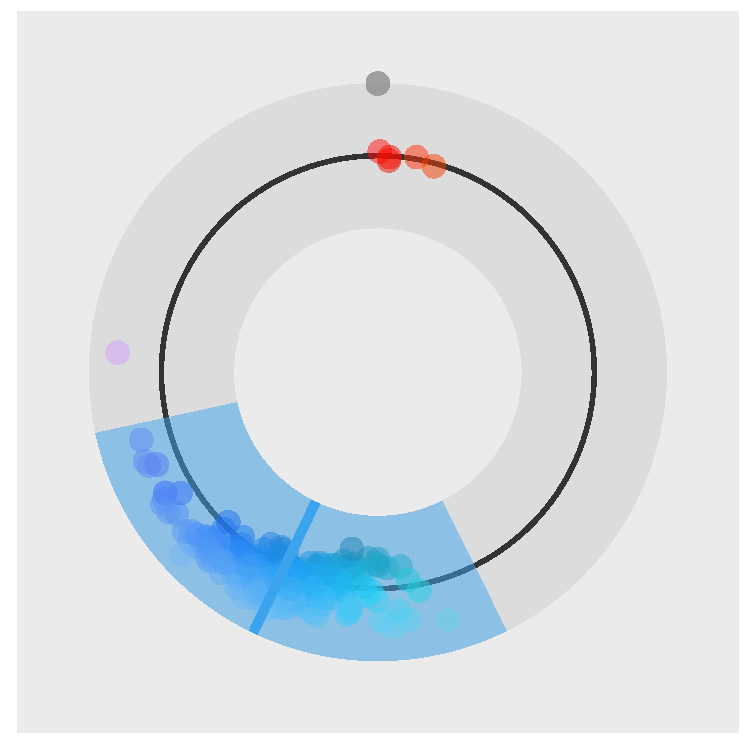
\includegraphics[width=\linewidth]{single_column.pdf}
%     \caption{\textbf{A random visualization.} This is an example of a figure that spans only across one of the two columns.}
%     \label{fig:column}
% \end{figure}

% On the other hand, \figurename~\ref{fig:whole} is an example of a figure that spans across the whole page (across both columns) of the report.

% \begin{figure*} makes the figure take up the entire width of the page
% \begin{figure*}[ht]\centering
%     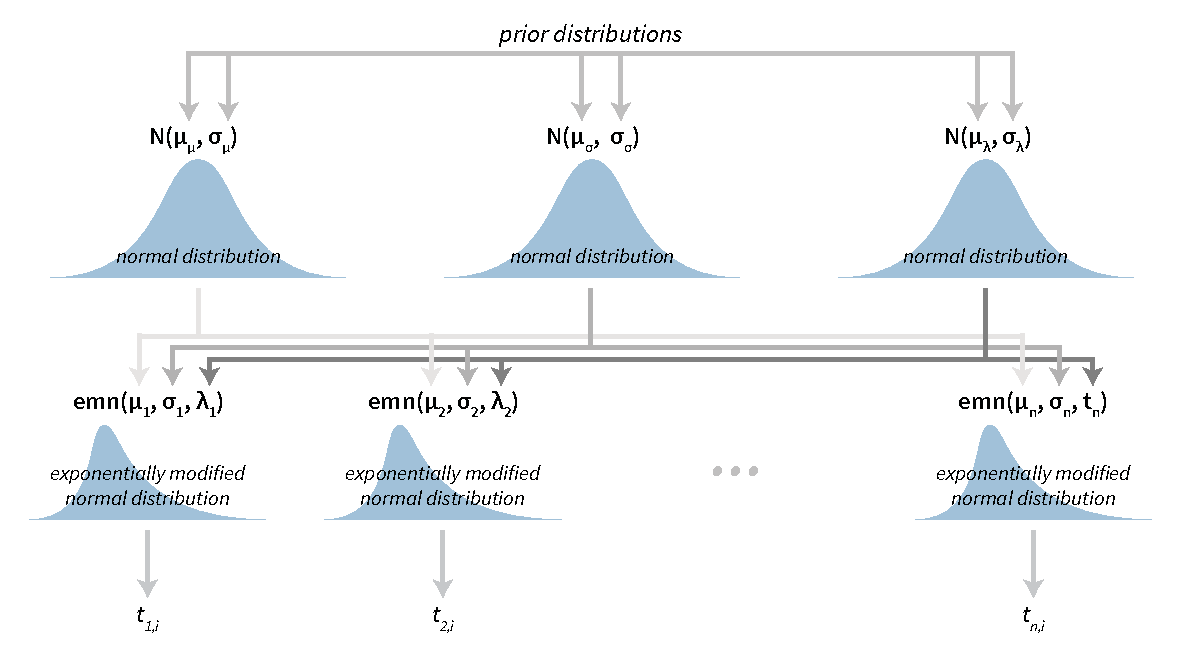
\includegraphics[width=\linewidth]{whole_page.pdf}
%     \caption{\textbf{Visualization of a Bayesian hierarchical model.} This is an example of a figure that spans the whole width of the report.}
%     \label{fig:whole}
% \end{figure*}


% \subsection*{Tables}

% Use the table environment to insert tables.

% \begin{table}[hbt]
%     \caption{Table of grades.}
%     \centering
%     \begin{tabular}{l l | r}
%         \toprule
%         \multicolumn{2}{c}{Name}       \\
%         \cmidrule(r){1-2}
%         First name & Last Name & Grade \\
%         \midrule
%         John       & Doe       & $7.5$ \\
%         Jane       & Doe       & $10$  \\
%         Mike       & Smith     & $8$   \\
%         \bottomrule
%     \end{tabular}
%     \label{tab:label}
% \end{table}


% \subsection*{Code examples}

% You can also insert short code examples. You can specify them manually, or insert a whole file with code. Please avoid inserting long code snippets, advisors will have access to your repositories and can take a look at your code there. If necessary, you can use this technique to insert code (or pseudo code) of short algorithms that are crucial for the understanding of the manuscript.

% \lstset{language=Python}
% \lstset{caption={Insert code directly from a file.}}
% \lstset{label={lst:code_file}}
% \lstinputlisting[language=Python]{code/example.py}

% \lstset{language=R}
% \lstset{caption={Write the code you want to insert.}}
% \lstset{label={lst:code_direct}}
% \begin{lstlisting}
% import(dplyr)
% import(ggplot)

% ggplot(diamonds,
% 	   aes(x=carat, y=price, color=cut)) +
%   geom_point() +
%   geom_smooth()
% \end{lstlisting}

%------------------------------------------------

% \section*{Results}

% Use the results section to present the final results of your work. Present the results in a objective and scientific fashion. Use visualisations to convey your results in a clear and efficient manner. When comparing results between various techniques use appropriate statistical methodology.

% \subsection*{More random text}

% This text is inserted only to make this template look more like a proper report. Lorem ipsum dolor sit amet, consectetur adipiscing elit. Etiam blandit dictum facilisis. Lorem ipsum dolor sit amet, consectetur adipiscing elit. Interdum et malesuada fames ac ante ipsum primis in faucibus. Etiam convallis tellus velit, quis ornare ipsum aliquam id. Maecenas tempus mauris sit amet libero elementum eleifend. Nulla nunc orci, consectetur non consequat ac, consequat non nisl. Aenean vitae dui nec ex fringilla malesuada. Proin elit libero, faucibus eget neque quis, condimentum laoreet urna. Etiam at nunc quis felis pulvinar dignissim. Phasellus turpis turpis, vestibulum eget imperdiet in, molestie eget neque. Curabitur quis ante sed nunc varius dictum non quis nisl. Donec nec lobortis velit. Ut cursus, libero efficitur dictum imperdiet, odio mi fermentum dui, id vulputate metus velit sit amet risus. Nulla vel volutpat elit. Mauris ex erat, pulvinar ac accumsan sit amet, ultrices sit amet turpis.

% Phasellus in ligula nunc. Vivamus sem lorem, malesuada sed pretium quis, varius convallis lectus. Quisque in risus nec lectus lobortis gravida non a sem. Quisque et vestibulum sem, vel mollis dolor. Nullam ante ex, scelerisque ac efficitur vel, rhoncus quis lectus. Pellentesque scelerisque efficitur purus in faucibus. Maecenas vestibulum vulputate nisl sed vestibulum. Nullam varius turpis in hendrerit posuere.

% Nulla rhoncus tortor eget ipsum commodo lacinia sit amet eu urna. Cras maximus leo mauris, ac congue eros sollicitudin ac. Integer vel erat varius, scelerisque orci eu, tristique purus. Proin id leo quis ante pharetra suscipit et non magna. Morbi in volutpat erat. Vivamus sit amet libero eu lacus pulvinar pharetra sed at felis. Vivamus non nibh a orci viverra rhoncus sit amet ullamcorper sem. Ut nec tempor dui. Aliquam convallis vitae nisi ac volutpat. Nam accumsan, erat eget faucibus commodo, ligula dui cursus nisi, at laoreet odio augue id eros. Curabitur quis tellus eget nunc ornare auctor.

% Phasellus in ligula nunc. Vivamus sem lorem, malesuada sed pretium quis, varius convallis lectus. Quisque in risus nec lectus lobortis gravida non a sem. Quisque et vestibulum sem, vel mollis dolor. Nullam ante ex, scelerisque ac efficitur vel, rhoncus quis lectus. Pellentesque scelerisque efficitur purus in faucibus. Maecenas vestibulum vulputate nisl sed vestibulum.


%------------------------------------------------

% \section*{Discussion}

% Use the Discussion section to objectively evaluate your work, do not just put praise on everything you did, be critical and exposes flaws and weaknesses of your solution. You can also explain what you would do differently if you would be able to start again and what upgrades could be done on the project in the future.


%------------------------------------------------

% \section*{Acknowledgments}

% Here you can thank other persons (non-authors) that contributed to the successful completion of your project.


%----------------------------------------------------------------------------------------
%	REFERENCE LIST
%----------------------------------------------------------------------------------------
\bibliographystyle{unsrt}
\bibliography{report}


\end{document}
